\documentclass{beamer}
\usepackage[british]{babel}
\usepackage{graphics,hyperref,url}
\usepackage{amsmath}
%\usepackage[linesnumbered,ruled,vlined]{algorithm2e}
\usepackage{algpseudocode}
\usepackage{algorithm}
\usepackage{algorithmicx}
\usepackage{tikz-qtree}
%\usepackage{algorithm2e,float}
\MakeRobust{\Call}
\usetheme{Boadilla}
% title of the presentation
% - first a short version which is visible at the bottom of each slide;
% - second the full title shown on the title slide;
\title[Tail Recursion Elimination]{Tail Recursion Elimination}
\subtitle{Recursive to iterative transformation}
% Tha author of the presentation:
% - again first a short version to be displayed at the bottom;
% - next the full list of authors, which may include contact information;
\author[Lucas M. Magliarelli]{
	Lucas M. Magliarelli 
}

% The institute:
% - to start the name of the university as displayed on the top of each slide
%   this can be adjusted such that you can also create a Dutch version
% - next the institute information as displayed on the title slide
\institute[TradeHelm Inc.]{
	TradeHelm Inc.
}
% add a date and possibly the name of the event to the slides
% - again first a short version to be shown at the bottom of each slide
% - second the full date and event name for the title slide
\date[March, 2018]{
	the 1st. presentation 2018
}
\begin{document}
\tikzset{every tree node/.style={minimum width=2em,draw,circle},
	blank/.style={draw=none},
	edge from parent/.style={draw,edge from parent path={(\tikzparentnode) -- (\tikzchildnode)}},
	level distance=1.5cm}
\begin{frame}
	\titlepage
\end{frame}
\begin{frame}
	\frametitle{Outline}
	\tableofcontents
\end{frame}
\section{Introduction}
\begin{frame}
	\frametitle{Introduction}
	Recursive programs are usually very descriptive, easy to code and to understand. However, they can have some issues:
	\begin{itemize}
		\item Recursive programs are executed by computers and computers have limitations
		\item Recursion, in computers, is implemented by using a stack
		\item a Stack is a portion of memory of fixed length. This sets a limit in the amount of invocations of the recursive calls. When such limit is reached, \texttt{StackOverflowException} is thrown
		\item Besides, every recursive call has to push their parameters and local variables into the stack and this is expensive
		\item Some recursive algorithms repeat calculations, that is, the recursive call is invoked with the same parameters many times. The running time of such algorithms are usually exponential. 
	\end{itemize}
\end{frame}
\section{Tail Recursion}
\begin{frame}
	\frametitle{Tail Recursion}
	\begin{block}{Tail Recursion}
		Tail recursion is a special kind of recursion where the recursive call is the very last thing in the function. It's a function that does not do anything at all after recursing.
		\begin{center}
				\begin{algorithmic}[1]
					\Procedure{recurse}{$p_0,p_1,\ldots,p_{n-1}$}
					\If{$g(p_0,p_1,\ldots,p_{n-1})$}
					\State\Return{$c$}
				\Else
					\State\Return{\Call{recurse}{$p_0',p_1',\ldots,p_{n-1}'$}}
				\EndIf
				\EndProcedure
			\end{algorithmic}
		\end{center}
	\end{block}
\end{frame}
\begin{frame}
	\frametitle{Tail Recursion}
	\begin{block}{Example}
				\begin{algorithmic}[1]
					\Procedure{gcd}{$a,b$}
					\If{$b=0$}
					\State\Return{$a$}
				\Else
					\State\Return{\Call{gcd}{$b,a$ mod $b$}}
				\EndIf
				\EndProcedure
			\end{algorithmic}
	\end{block}
\end{frame}
\section{Linear Recursion}
\begin{frame}
	\frametitle{Linear Recursion}
	\begin{block}{Linear Recursion}
		A linear recursive function is a function that only makes a single call to itself each time the function runs, and th recusive call is not the last operation in the function
				\begin{algorithmic}[1]
					\Procedure{recurse}{$p_0,p_1,\ldots,p_{n-1}$}
					\If{$g(p_0,p_1,\ldots,p_{n-1})$}
					\State\Return{$c$}
				\Else
					\State\Return{$f$(\Call{recurse}{$p_0',p_1',\ldots,p_{n-1}'$})}
				\EndIf
				\EndProcedure
			\end{algorithmic}
	\end{block}
\end{frame}

\begin{frame}
	\frametitle{Linear Recursion}
	\begin{block}{Example}
				\begin{algorithmic}[1]
					\Procedure{factorial}{$n$}
					\If{$n=0$}
					\State\Return{$1$}
				\Else
					\State\Return{$n\times$ \Call{factorial}{$n-1$}}
				\EndIf
				\EndProcedure
			\end{algorithmic}
	\end{block}
\end{frame}
\section{Multiple recursion}
\begin{frame}
	\frametitle{Multiple Recursion}
	\begin{block}{Multiple Recursion}
		A multiple recursive function is like a \textit{Linear recursive} function, but there are more than one calls to itself.
				\begin{algorithmic}[1]
					\Procedure{recurse}{$p_0,p_1,\ldots,p_{n-1}$}
					\If{$g(p_0,p_1,\ldots,p_{n-1})$}
					\State\Return{$c$}
				\Else
					\State\Return{$f$(\Call{recurse}{$p_0^0,p_1^0,\ldots,p_{n-1}^0$}, \Call{recurse}{$p_0^1,p_1^1,\ldots,p_{n-1}^1$},$\ldots$, \Call{recurse}{$p_0^{m-1},p_1^{m-1},\ldots,p_{n-1}^{m-1}$})}
				\EndIf
				\EndProcedure
			\end{algorithmic}
	\end{block}
\end{frame}
\begin{frame}
	\frametitle{Multiple Recursion}
	\begin{block}{Example}
			\begin{algorithmic}[1]
				\Procedure{fibonacci}{$n$}
				\If{$n=0$}
					\State\Return{$0$}
				\Else
					\If{$n=1$}
						\State\Return{$1$}
					\Else
						\State\Return{\Call{fibonacci}{$n-1$} +  \Call{fibonacci}{$n-2$}}
					\EndIf
				\EndIf
				\EndProcedure
			\end{algorithmic}
	\end{block}
\end{frame}
\section{Nested Recursion}
\begin{frame}
	\frametitle{Nested Recursion}
	\begin{block}{Nested Recursion}
		In nested recursion, one of the arguments to the recursive function is the recursive function itself. These functions tend to grow extremely fast. A good example is the classic mathematical function: \textit{Ackermann's function}. It grows very quickly (even for small values of $x$ and $y$, $ackermann(x,y)$ is extremely large) and it cannot be computed with only definite iteration; it requires indefinite iteration 
			\begin{algorithmic}[1]
				\Procedure{recurse}{$x,y$}
				\If{$g(x,y)$}
					\State\Return{$c$}
				\Else
					\State\Return{\Call{recurse}{$x'$,\Call{recurse}{$x''$, $y''$}}}
				\EndIf
				\EndProcedure
			\end{algorithmic}
	\end{block}
\end{frame}
\begin{frame}
	\frametitle{Nested Recursion}
	\begin{block}{Example}
			\begin{algorithmic}[1]
				\Procedure{ackermann}{$x,y$}
				\If{$x=0$}
					\State\Return{$y+1$}
				\Else
					\If{$y=0$}
						\State\Return{\Call{ackermann}{$x-1,1$}}
					\Else
						\State\Return{\Call{ackermann}{$x-1$,\Call{ackermann}{$x$, $y-1$}}}
					\EndIf
				\EndIf
				\EndProcedure
			\end{algorithmic}
	\end{block}
\end{frame}

\section{Recursive to iterative transformation}

\begin{frame}
	\frametitle{Recursive to iterative transformation}
	\begin{itemize}
		\item \textit{Tail recursion} is the easiest one to convert to iterative. We only have to iterate over the parameters until we get to the \textit{base case}.
		\item \textit{Linear Recursion}, we have to convert the \textit{Linear Recursive} fucntion to a \textit{Tail Recursive} function. This is generally carried out by adding a new parameter to the function, which acts as an \textit{accumulator}
		\item \textit{Nested Recursion} is generally converted to a \textit{Tail Recursion} form by adding a \textit{Stack} to its parameters and using the \textit{fold/unfold} technique.
		\item \textit{Multiple Recursion} is usually converted to a \textit{Nested Recursion} form by adding a new parameter and generalizing its \textit{range}, that is, what it returns. We already know how to convert a \textit{Nested Recursion} form to a \textit{Tail Recursion} form
	\end{itemize}
\end{frame}
\begin{frame}
	\frametitle{Tail Recursion to Iterative Transformation}
	Let's convert recursive \textit{GCD} to an iterative version.
	\begin{block}{Recursive Version}
				\begin{algorithmic}[1]
					\Procedure{gcd}{$a,b$}
					\If{$b=0$}
					\State\Return{$a$}
				\Else
					\State\Return{\Call{gcd}{$b,a$ mod $b$}}
				\EndIf
				\EndProcedure
			\end{algorithmic}
	\end{block}	
\end{frame}
\begin{frame}
	\frametitle{Tail Recursion to Iterative Transformation}
	Let's convert recursive \textit{GCD} to an iterative version.
	\begin{block}{Iterative Version}
				\begin{algorithmic}[1]
					\Procedure{iterative-gcd}{$a,b$}
					\While{$b\neq0$}
						\State $tmp \gets a$ \Comment {We save $a$ temporally since we need its value to update $b$}
						\State $a\gets b$
						\State $b \gets $ $tmp$ $mod$ $b$
					\EndWhile
					\State\Return{$a$}
				\EndProcedure
			\end{algorithmic}
	\end{block}	
\end{frame}
\begin{frame}
	\frametitle{Tail Recursion to Iterative Transformation}
	As you see the transformation is straightforward. There are two differences:
	\begin{itemize}
		\item We use $b\neq 0$ in the \textbf{while} condition since the iteration is to simulate the recursive call
		\item We introduce the $tmp$ variable to keep the current value of $a$ which is needed to update $b$ for the next iteration.
	\end{itemize}
\end{frame}
\begin{frame}
	\frametitle{Linear Recursion to Iterative Transformation}
	Now, we will transform \textit{factorial} recursive version into an iterative one.
	\begin{block}{Recursive Version}
				\begin{algorithmic}[1]
					\Procedure{factorial}{$n$}
					\If{$n=0$}
					\State\Return{$1$}
				\Else
					\State\Return{$n\times$ \Call{factorial}{$n-1$}}
				\EndIf
				\EndProcedure
			\end{algorithmic}
	\end{block}
\end{frame}
\begin{frame}
	\frametitle{Linear Recursion to Iterative Transformation}
	To do so, we first have to transform it to a \textit{Tail Recursion} version. We will do this by proposing a new function which for some initial values of its parameters it is the same as \textit{factorial}. In this case, we will add a new $m$ parameter. This will be an integer and it will accumulate $n\times n-1\times n-2\times \ldots$
	\begin{block}{Recursive Version}
			\begin{algorithmic}[1]
				\Procedure{t-factorial}{$n,m$}
					\State\Return{$m \times$ \Call{factorial}{$n$}}
				\EndProcedure
			\end{algorithmic}
	\end{block}
\end{frame}
\begin{frame}
	\frametitle{Linear Recursion to Iterative Transformation}
	Let's \textbf{unfold} the definition of \textit{factorial(n)}
	\begin{block}{Unfolding...}
		\begin{algorithmic}[1]
			\Procedure{t-factorial}{$n,m$}
			\If{$n = 0$}
				\State\Return{$m \times 1$}
			\Else
				\State\Return{$m\times n\times$\Call{factorial}{$n-1$}}
			\EndIf
			\EndProcedure
		\end{algorithmic}
	\end{block}
\end{frame}
\begin{frame}
	\frametitle{Linear Recursion to Iterative Transformation}
	If we take a closer look at $m \times n \times factorial(n-1)$ and we use the associative property of multiplication operation, we have this $(m\times n) \times factorial(n-1)$. Now, by the definition of $t-factorial$, 
	\begin{equation}
		(m\times n) \times factorial(n-1) = t-factorial(n-1,m \times n)
	\end{equation}
	This is called \textbf{fold}, which is the inversion of \textbf{unfold}.
	\begin{itemize}
		\item \textbf{fold} means replacing the expression definition by its function invocation
		\item \textbf{unfold} means replacing the function invocation by its definition
	\end{itemize}
\end{frame}
\begin{frame}
	\frametitle{Linear Recursion to Iterative Transformation}
	We finally got a \textit{Tail Recursive} version
	\begin{block}{Tail Recursive Version} 
		\begin{algorithmic}[1]
			\Procedure{t-factorial}{$n,m$}
			\If{$n = 0$}
				\State\Return{$m \times 1$}
			\Else
				\State\Return{\Call{t-factorial}{$n-1, m \times n$}}
			\EndIf
			\EndProcedure
		\end{algorithmic}
	\end{block}
\end{frame}
\begin{frame}
	\frametitle{Linear Recursion to Iterative Transformation}
	\begin{block}{Iterative Version of $t-factorial$}
		\begin{algorithmic}[1]
			\Procedure{iterative-t-factorial}{$n,m$}
			\While{$n \neq 0$}
				\State $m \gets m \times n$
				\State $n \gets n-1$
			\EndWhile
			\State\Return{$m$}
			\EndProcedure
		\end{algorithmic}
	\end{block}
\end{frame}
\begin{frame}
	\frametitle{Linear Recursion to Iterative Transformation}
	\textit{iterative-t-factorial} is a function such that its range is larger than the range of \textit{factorial} function, but it includes \textit{factorial} range. We said at the beginning that both functions will be the same for some initial parameters value. In this case, such parameter value if $m = 1$. Thus, our \textit{iterative-factorial} is
	\begin{block}{Iterative Version of $factorial$}
		\begin{algorithmic}[1]
			\Procedure{iterative-factorial}{$n$}
			\State\Return{\Call{iterative-t-factorial}{$n,1$}}
			\EndProcedure
		\end{algorithmic}
	\end{block}
\end{frame}
\begin{frame}
	\frametitle{Nested Recursion to Iterative Transformation}
	Now, we will try to tranform our recursive \textit{Ackermann} function into an iterative one. To do so, we will propose a new function such that for some intial values of its parameters, it will equal to \textit{Ackermann}. This new function will replace the \textit{Ackermann}'s first parameter $x$ with an \textit{Stack} $p$. Besides, this new function is \textit{Tail Recursive}
	\begin{block}{Recursive version}
		\begin{algorithmic}[1]
			\Procedure{t-ackermann}{$p,y$}
				\If{$isEmpty(p)$}
					\State\Return{$y$}
				\Else
					\State\Return{\Call{t-ackermann}{$pop(p)$,\Call{ackermann}{$top(p),y$}}}
				\EndIf
			\EndProcedure
		\end{algorithmic}
	\end{block}
\end{frame}
\begin{frame}
	\frametitle{Nested Recursion to Iterative Transformation}
	Let's now \textbf{unfold} \textit{ackermann}
	\begin{block}{Unfolding...}
		\begin{algorithmic}[1]
			\tiny
			\Procedure{t-ackermann}{$p,y$}
				\If{$isEmpty(p)$}
					\State\Return{$y$}
				\Else
					\If{$top(p) = 0$}
						\State\Return{\Call{t-ackermann}{$pop(p),y+1$}}
					\Else
						\If{$y = 0$}
							\State\Return{\Call{t-ackermann}{$pop(p)$,\Call{ackermann}{$top(p)-1,1$}}}
						\Else
							\State\Return{\Call{t-ackermann}{$pop(p)$, \Call{ackermann}{$top(p)-1$,\Call{ackermann}{$top(p), y-1$}}}}
						\EndIf
					\EndIf
				\EndIf
			\EndProcedure
		\end{algorithmic}
	\end{block}
\end{frame}

\begin{frame}
	\frametitle{Nested Recursion to Iterative Transformation}
	We now have three recursive calls.
	\begin{itemize}
		\item the first one is in line number $6$. It is \textit{Tail Recursive}. We don't have to do anything here.
		\item the second one is in line number $9$. It is \textit{Tail Recursive}, but it still contains an invocation to \textit{ackermann} function. We have to get rid of this invocation
		\item the third one is in line number $11$. It is also \textit{Tail Recursive}, but it still contains a \textit{Nested} invocation to \textit{ackermann} function. We have to get rid of these invocations too.
	\end{itemize}
\end{frame}
\begin{frame}
	\frametitle{Nested Recursion to Iterative Transformation}
	Now, we will convert line number $6$ into a \textit{Tail Recursive} form without any reference to \textit{ackermann}.\\ This line looks like the line number $5$ in our \textit{t-ackermann} definition. Thus, we can \textbf{fold} it and we get this:
	\begin{equation}
		\begin{split}
		t-ackermann(pop(p),ackermann(top(p)-1,1)) \\ = t-ackermann(push(top(p)-1,pop(p)),1)
		\end{split}
	\end{equation}

\end{frame}
\begin{frame}
	\frametitle{Nested Recursion To Iterative Transformation} 
	Finally, we will convert line $11$ to a \textit{Tail Recursive} form. We will do this by \textbf{folding} the expression two times.
	\begin{equation}
		\begin{split}
			t-ackermann(pop(p),ackermann(top(p)-1,ackermann(top(p),y-1))) \\ =
			t-ackermann(push(top(p)-1,pop(p)),ackermann(top(p),y-1))\\  = 
			t-ackermann(push(top(p),push(top(p)-1,pop(p))), y-1)
		\end{split}
	\end{equation}
\end{frame}
\begin{frame}
	\frametitle{Nested Recursion to Iterative Transformation}
	Let's rewrite \textit{t-ackermann} by replacing the lines $6$ and $11$ 
	\begin{block}{Folding...}
		\begin{algorithmic}[1]
			\tiny
			\Procedure{t-ackermann}{$p,y$}
				\If{$isEmpty(p)$}
					\State\Return{$y$}
				\Else
					\If{$top(p) = 0$}
						\State\Return{\Call{t-ackermann}{$pop(p),y+1$}}
					\Else
						\If{$y = 0$}
							\State\Return{\Call{t-ackermann}{$push(top(p)-1,pop(p)),1$}}
						\Else
							\State\Return{\Call{t-ackermann}{$push(top(p),push(top(p)-1,pop(p))),y-1$}}
						\EndIf
					\EndIf
				\EndIf
			\EndProcedure
		\end{algorithmic}
	\end{block}
\end{frame}
\begin{frame}
	\frametitle{Nested Recursion To Iterative Transformation}
	It is time to write our iterative version for \textit{t-ackermann}
	\begin{block}{Iterative $t-ackermann$}
		\begin{algorithmic}[1]
			\tiny
			\Procedure{iterative-t-ackermann}{$p,y$}
			\While {$\neg isEmpty(p)$}
				\State $t \gets top(p)$
				\State $p \gets pop(p)$
				\If{$t = 0$}
					\State $y\gets y+1$
				\Else
					\If {$y = 0$}
						\State $y \gets 1$
						\State $p \gets push(t-1,p) $
					\Else
						\State $y \gets y-1$
						\State $p \gets push(t-1,p)$
						\State $p \gets push(t,p)$
					\EndIf
				\EndIf
			\EndWhile
			\State\Return{$y$}
			\EndProcedure
		\end{algorithmic}
	\end{block}
\end{frame}
\begin{frame}
	\frametitle{Nested Recursion To Iterative Transformation}
	Lastly, we will write out iterative \textit{ackermann}. To do so, we have to provide $t-ackermann$ with the proper initial parameters so that it computes \textit{ackermann}. If we invoke \textit{t-ackermann} with 
	\begin{itemize}
		\item $p = push(x, [])$
		\item $y = y$
	\end{itemize}
	we will have this - by using our very first definition of $t-ackermann$
	\begin{equation}
		\begin{split}
		t-ackermann(push(x,[]), y)\\ = t-ackermann([], ackermann(x,y))\\ = ackermann(x,y)
		\end{split}
	\end{equation}
	Then..
	\begin{block}{Iterative $ackermann$}
		\begin{algorithmic}[1]
			\Procedure{iterative-ackermann}{$x,y$}
				\State $p \gets push(x, [])$
				\State\Return {\Call{iterative-t-ackermann}{p,y}}
			\EndProcedure
		\end{algorithmic}
	\end{block}
\end{frame}
\begin{frame}
	\frametitle{Multiple Recursive to Iterative Transformation}
	To convert our \textit{fibonacci} recursive function, we first have to find a new recursive function that calculates \textit{fibonacci} for some parameters and it is a \textit{Nested Recursive} function. Let's try this:
	\begin{block}{Nested Version of $fibonacci$}
		\begin{algorithmic}[1]
			\Procedure{nested-fibonacci}{$n,m$}
				\State\Return{$m +$ \Call{fibonacci}{n}}
			\EndProcedure
		\end{algorithmic}
	\end{block}
\end{frame}
\begin{frame}
	\frametitle{Multiple Recursive to Iterative Transformation}
	Let's \textbf{unfold} \textit{fibonacci}
	\begin{block}{Unfolding...}
		\begin{algorithmic}[1]
			\Procedure{nested-fibonacci}{$n,m$}
				\If{$n = 0$}
					\State\Return{$m+0$}
				\Else
					\If{$n=1$}
						\State\Return{$m+1$}
					\Else
						\State\Return{$m+$\Call{fibonacci}{$n-1$}+\Call{fibonacci}{$n-2$}}
					\EndIf
				\EndIf
			\EndProcedure
		\end{algorithmic}
	\end{block}
\end{frame}
\begin{frame}
	\frametitle{Multiple Recursive to Iterative Transformation}
	If we now associate $m + fibonacci(n-1)$ and we call it $m'$, then line $8$ looks like $m' + fibonacci(n-2)$. We ca \textbf{fold} this. 
	\begin{equation}
		\begin{split}
		m' + fibonacci(n-2) = nested-fibonacci(n-2,m') \\ =
		nested-fibonacci(n-2, m + fibonacci(n-1))
		\end{split}
	\end{equation}
	We can also \textbf{fold} $m + fibonacci(n-1)$ which it is equal to $nested-fibonacci(n-1,m)$
\end{frame}
\begin{frame}
	\frametitle{Multiple Recursive to Iterative Tansformation}
	\begin{block}{Folding...}
		\begin{algorithmic}[1]
			\tiny
			\Procedure{nested-fibonacci}{$n,m$}
				\If{$n = 0$}
					\State\Return{$m+0$}
				\Else
					\If{$n=1$}
						\State\Return{$m+1$}
					\Else
						\State\Return{\Call{nested-fibonacci}{$n-2$, \Call{nested-fibonacci}{$n-1,m$}}}
					\EndIf
				\EndIf
			\EndProcedure
		\end{algorithmic}
	\end{block}
\end{frame}
\begin{frame}
	\frametitle{Multiple Recursive to Iterative Transformation}
	Now, it is time to convert \textit{nested-fibonacci} into \textit{tail-fibonacci}. To do so, we propouse this new function. Again, we will use a \textit{Stack} $p$
	\begin{block}{$tail-fibonacci$}
		\begin{algorithmic}[1]
			\small 
			\Procedure{tail-fibonacci}{$p,m$}
				\If{$isEmpty(p)$}
					\State\Return{$m$}
				\Else
					\State\Return{\Call{tail-fibonacci}{$pop(p)$,\Call{nested-fibonacci}{$top(p),m$}}}
				\EndIf
			\EndProcedure
		\end{algorithmic}
	\end{block}
\end{frame}
\begin{frame}
	\frametitle{Multiple Recursive to Iterative Transformation}
	Let's \textbf{unfold} \textit{nested-fibonacci}
	\begin{block}{Unfolding...}
		\tiny
		\begin{algorithmic}[1]
			\Procedure{tail-fibonacci}{$p,m$}
				\If {$isEmpty(p)$}
					\State\Return{$m$}
				\Else
					\If{$top(p) = 0$}
						\State\Return{\Call{tail-fibonaci}{$pop(p), m$}}
					\Else
						\If{$top(p) = 1$}
							\State\Return{\Call{tail-fibonacci}{$pop(p),m+1$}}
						\Else
							\State\Return{\Call{tail-fibonacci}{$pop(p)$, \Call{nested-fibonacci}{$n-2$,\Call{nested-fibonacci}{$n-1,m$}}}}
						\EndIf
					\EndIf
				\EndIf
			\EndProcedure
		\end{algorithmic}
	\end{block}
\end{frame}
\begin{frame}
	\frametitle{Multiple Recursive to Iterative Transformation}
	We only have to take care of line $11$. By using our \textit{tail-fibonacci} definition, we will be able to \textbf{fold} two times line $11$.
	\begin{equation}
		\tiny
		\begin{split}
			tail-fibonacci(pop(p),nested-fibonacci(n-2,nested-fibonacci(n-1,m))) \\ =
			tail-fibonacci(push(n-2,pop(p)),nested-fibonacci(n-1,m))\\ =
			tail-fibonacci(push(n-1,push(n-2,pop(p))),m)
		\end{split}
	\end{equation}
\end{frame}
\begin{frame}
	\frametitle{Multiple Recursive to Iterative Transformation}
	Let's \textbf{fold} \textit{nested-fibonacci}
	\begin{block}{Folding...}
		\tiny
		\begin{algorithmic}[1]
			\Procedure{tail-fibonacci}{$p,m$}
				\If {$isEmpty(p)$}
					\State\Return{$m$}
				\Else
					\If{$top(p) = 0$}
						\State\Return{\Call{tail-fibonaci}{$pop(p), m$}}
					\Else
						\If{$top(p) = 1$}
							\State\Return{\Call{tail-fibonacci}{$pop(p),m+1$}}
						\Else
							\State\Return{\Call{tail-fibonacci}{$push(n-1,push(n-2,pop(p)))$, $m$}}
						\EndIf
					\EndIf
				\EndIf
			\EndProcedure
		\end{algorithmic}
	\end{block}
\end{frame}
\begin{frame}
	\frametitle{Multiple Recursive to Iterative Transformation}
	We can now convert \textit{tail-fibonacci} into an \textit{iterative} one.
	\begin{block}{Iterative Fibonacci - 1}
		\begin{algorithmic}[1]
			\Procedure{iterative-fibonacci-1}{$p,m$}
				\While{$\neg isEmpty(p)$}
					\State $t \gets top(p)$
					\State $p \gets pop(p)$
					\If{$t \neq 0$}
					\If {$t = 1$}
						\State $m \gets m+1$
					\Else
						\State $p \gets push(n-2,p)$
						\State $p \gets push(n-1,p)$
					\EndIf
					\EndIf
				\EndWhile
				\State\Return{$m$}
			\EndProcedure
		\end{algorithmic}
	\end{block}
\end{frame}
\begin{frame}
	\frametitle{Multiple Recursive to Iterative Transformation}
	Our final iterative version of \textit{fibonacci} is defined by invoking \textit{iterative-fibonacci-1} with the proper arguments. Those arguments are the ones that make \textit{nested-fibonacci} return \textit{fibonacci}. Those are
	\begin{itemize}
		\item $p = push(n,[])$
		\item $m = 0$
	\end{itemize}
	\begin{block}{Iterative Fibonacci}
		\begin{algorithmic}[1]
			\Procedure{iterative-fibonacci}{$n$}
				\State $p \gets push(n,[])$
				\State\Return{\Call{iterative-fibonacci-1}{p,0}}
			\EndProcedure
		\end{algorithmic}
	\end{block}
\end{frame}
\begin{frame}
	\frametitle{Multiple Recursive to Iterative Transformation}
	We finally got an interative version of \textit{fibonacci}, but it has two drawbacks.
	\begin{itemize}
		\item It's implementation is more complex than the naive iterative version we all know.
			\begin{block}{Naive Iterative version}
				\begin{algorithmic}[1]
					\tiny
					\Procedure{naive-iterative-fibonacci}{$n$}
						\State $a \gets 0$
						\State $b \gets 1$
						\If {$n = 0$}
							\State $ b \gets 0$
						\Else				
							\While {$n > 1$}
								\State $tmp \gets b$
								\State $b \gets a + b$
								\State $a \gets temp$
								\State $n \gets n-1$							
							\EndWhile
						\EndIf
						\State \Return{$b$}
					\EndProcedure
				\end{algorithmic}
			\end{block}
		\item The running time of this version is still exponential- $\Theta(\frac{1+\sqrt(5)}{2}^n)$-, since for each number calculated, it needs to calculate all the previous numbers more than once. 
	\end{itemize}
\end{frame}
\begin{frame}
	\begin{center}
	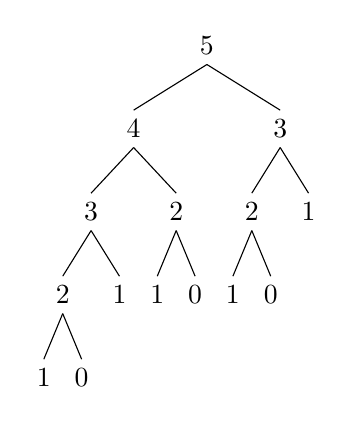
\begin{tikzpicture}
		\Tree
		[.5
			[.4 
				[.3 
					[.2 
						[.1 ]
						[.0 ]
					]
					[.1 ]
				]
				[.2 
					[.1 ]
					[.0 ]
				]
			]
			[.3 				
				[.2 
					[.1 ]
					[.0 ]
				]
				[.1 ]
			]
		]
	\end{tikzpicture}
	\end{center}
\end{frame}
\begin{frame}
	\frametitle{Multiple Recursive to Iterative Transformation}
	Can we convert \textit{fibonacci} into a \textit{tail-recursive} function which it doesn't repeat invocations?. Yes, we can!\\
	How can we avoid recalculating values?. One way to do so is to extend the function range. The new function will return an ordered pair containing both $f(n+1)$ and $f(n)$. Thus, every time we need a previous value, it will be there.
	\begin{block}{g-fibonacci}
		\tiny
		\begin{algorithmic}[1]
			\Procedure{g-fibonacci}{$n$}
				\State\Return{$<$\Call{fibonacci}{$n+1$},\Call{fibonacci}{$n$}$>$}
			\EndProcedure
		\end{algorithmic}
	\end{block}
\end{frame}
\begin{frame}
	\frametitle{Multiple Recursive to Iterative Transformation}
	Let's \textbf{unfold} \textit{fibonacci(n)}.
	\begin{block}{g-fibonacci}
		\tiny
		\begin{algorithmic}[1]
			\Procedure{g-fibonacci}{$n$}
				\If {$n+1=1$}
					\State\Return{$<1,0>$}
				\Else
					\State\Return{$<$\Call{fibonacci}{$n$} + \Call{fibonacci}{$n-1$} ,\Call{fibonacci}{$n$}$>$}
				\EndIf
			\EndProcedure
		\end{algorithmic}
	\end{block}
	We know that for $n \geq 1$ $g-fibonacci(n-1)$ is 
	\begin{itemize}
		\item $<fibonacci(n),fibonacci(n-1)>$
	\end{itemize}
	using this we can replace
	\begin{itemize}
		\item $fibonacci(n) = g-fibonacci(n-1)_0$
		\item $fibonacci(n-1) = g-fibonacci(n-1)_1$
	\end{itemize}
\end{frame}
\begin{frame}
	\frametitle{Multiple Recursive to Iterative Transformation}
	Let's \textbf{fold}
	\begin{block}{g-fibonacci}
		\tiny
		\begin{algorithmic}[1]
			\Procedure{g-fibonacci}{$n$}
				\If {$n+1=1$}
					\State\Return{$<1,0>$}
				\Else
						\State\Return{$<$\Call{g-fibonacci}{$n-1$}$_0$ + \Call{g-fibonacci}{$n-1$}$_1$ ,\Call{g-fibonacci}{$n-1$}$_0$$>$}
				\EndIf
			\EndProcedure
		\end{algorithmic}
	\end{block}
	This new version only depends on $g-fibonacci(n-1)$. This avoids repeating calculation. Let's try to convert it to a \textit{Nested Recursive} version
\end{frame}
\begin{frame}
	\frametitle{Multiple Recursive to Iterative Transformation}
	\begin{block}{Nested Recursive}
		\begin{algorithmic}[1]
			\Procedure{gg-fibonacci}{$n,action,t$}
				\If {$action = done$}
					\State\Return {$t$}
				\Else
					\If {$action = build$}
						\State\Return{\Call{gg-fibonacci}{$n,done,<t_0+t_1,t_0>$}}
					\Else
						\State\Return{\Call{gg-fibonacci}{$n,done$,\Call{g-fibonacci}{$n$}}}
					\EndIf
				\EndIf
			\EndProcedure
		\end{algorithmic}
	\end{block}
\end{frame}
\begin{frame}
	\frametitle{Multiple Recursive to Iterative Transformation}
	\begin{block}{Unfolding $g-fibonacci$}
		\begin{algorithmic}[1]
			\tiny
			\Procedure{gg-fibonacci}{$n,action,t$}
				\If {$action = done$}
					\State \Return{$t$}
				\Else
					\If {$action = build$}
						\State\Return{\Call{gg-fibonacci}{$n,done,<t_0+t_1,t_0>$}}
					\Else
						\If {$ n+1 = 1$}
							\State\Return{\Call{gg-fibonacci}{$n,done,<1,0>$}}
						\Else
							\State\Return{\Call{gg-fibonacci}{$n,done$,$<$\Call{g-fibonacci}{$n-1$}$_0$ + \Call{g-fibonacci}{$n-1$}$_1$,\Call{g-fibonacci}{$n-1$}$_0>$}}
						\EndIf
					\EndIf
				\EndIf
			\EndProcedure
		\end{algorithmic}
	\end{block}
	\begin{equation}
		\tiny
		\begin{split}
			gg-fibonacci(n,done,<g-fibonacci(n-1)_0 + g-fibonacci(n-1)_1,g-fibonacci(n-1)_0>)\\=
			gg-fibonacci(n,build,g-fibonacci(n-1)) \\=
			gg-fibonacci(n,build,gg-fibonacci(n-1,process,t))
		\end{split}
	\end{equation}
\end{frame}
\begin{frame}
	\frametitle{Multiple Recursive to Iterative Transformation}
	\begin{block}{Folding...}
		\begin{algorithmic}[1]
			\tiny
			\Procedure{gg-fibonacci}{$n,action,t$}
				\If {$action = done$}
					\State \Return{$t$}
				\Else
					\If {$action = build$}
						\State\Return{\Call{gg-fibonacci}{$n,done,<t_0+t_1,t_0>$}}
					\Else
						\If {$ n+1 = 1$}
							\State\Return{\Call{gg-fibonacci}{$n,done,<1,0>$}}
						\Else
							\State\Return{\Call{gg-fibonacci}{$n,build$,\Call{gg-fibonacci}{$n-1,process,t$}}}
						\EndIf
					\EndIf
				\EndIf
			\EndProcedure
		\end{algorithmic}
	\end{block}
\end{frame}
\begin{frame}
	\frametitle{Multiple Recursive to Iterative Transformation}
	Now, it is time to convert this \textit{Nested Recursive} version into a \textit{Tail Recursive} one.
	\begin{block}{Tail Recursive Version}
		\tiny
		\begin{algorithmic}[1]
			\Procedure{ggg-fibonacci}{$p,t$}
				\If{$isEmpty(p)$}
					\State\Return{$t$}
				\Else
					\State\Return{\Call{ggg-fibonacci}{$pop(p)$, \Call{gg-fibonacci}{$top(p)_0,top(p)_1,t$}}}
				\EndIf
			\EndProcedure
		\end{algorithmic}
	\end{block}
\end{frame}
\begin{frame}
	\frametitle{Multiple Recursive to Iterative Transformation}
	Let's \textbf{unfold} $gg-fibonacci$
	\begin{block}{Tail Recursive Version}
		\tiny
		\begin{algorithmic}[1]
			\Procedure{ggg-fibonacci}{$p,t$}
				\If{$isEmpty(p)$}
					\State\Return{$t$}
				\Else
					\If {$top(p)_1 = done$}
						\State\Return{\Call{ggg-fibonacci}{$pop(p),t$}}
					\Else
						\If {$top(p)_1 = build$}
							\State\Return{\Call{ggg-fibonacci}{$pop(p)$,\Call{gg-fibonacci}{$top(p)_0,done,<t_0+t_1,t_0>$}}}
						\Else
							\If {$top(p)_0 + 1 = 1$}
								\State\Return{\Call{ggg-fibonacci}{$pop(p)$,\Call{gg-fibonacci}{$top(p)_0,done,<1,0>$}}}
							\Else
								\State\Return{\Call{ggg-fibonacci}{$pop(p)$,\Call{gg-fibonacci}{$top(p)_0,build,$,\Call{gg-fibonacci}{$top(p)_0-1,process,t$}}}}
							\EndIf
						\EndIf
					\EndIf
				\EndIf
			\EndProcedure
		\end{algorithmic}
	\end{block}
\end{frame}
\begin{frame}
	\frametitle{Multiple Recursive to Iterative Transformation}
	We have to \textbf{fold} lines $9$, $12$ and $14$. Let's see line $9$ and $12$ first.\\
	Since $done = true$ and by $gg-fibonacci$ definition  
	\begin{itemize}
		\item $gg-fibonacci(top(p)_0,done,<t_0+t_1,t_0>) = <t_0+t_1,t_0>$. 
		\item $gg-fibonacci(top(p)_0,done,<1,0>) = <1,0>$. 
	\end{itemize}
	Let's now see line $14$. We will use line number $5$ of $ggg-fibonacci$ definition to \textbf{fold}
	\begin{equation}
		\tiny
		\begin{split}
			ggg-fibonacci(pop(p),gg-fibonacci(top(p)_0,build,gg-fibonacci(top(p)_0-1,process,t))) \\=
			ggg-fibonacci(push(<top(p)_0,build>,pop(p)), gg-fibonacci(top(p)_0-1,process,t)) \\=
			ggg-fibonacci(push(<top(p)_0-1,process>,push(<top(p)_0,build>,pop(p))),t)
		\end{split}
	\end{equation}

\end{frame}
\begin{frame}
	\frametitle{Multiple Recursive to Iterative Transformation}
	\begin{block}{Tail Recursive Version - fold}
		\tiny
		\begin{algorithmic}[1]
			\Procedure{ggg-fibonacci}{$p,t$}
				\If{$isEmpty(p)$}
					\State\Return{$t$}
				\Else
					\If {$top(p)_1 = done$}
						\State\Return{\Call{ggg-fibonacci}{$pop(p),t$}}
					\Else
						\If {$top(p)_1 = build$}
							\State\Return{\Call{ggg-fibonacci}{$pop(p),<t_0+t_1,t_0>$}}
						\Else
							\If {$top(p)_0+1 = 1$}

								\State\Return{\Call{ggg-fibonacci}{$pop(p),<1,0>$}}
							\Else
								\State\Return{\Call{ggg-fibonacci}{$push(<top(p)_0-1,process>,push(<top(p)_0,build>,pop(p))),t$}}
							\EndIf
						\EndIf
					\EndIf
				\EndIf
			\EndProcedure
		\end{algorithmic}
	\end{block}
\end{frame}
\begin{frame}
	\frametitle{Multiple Recursive to Iterative Transformation}
	\begin{block}{Iterative version}
		\begin{algorithmic}[1]
			\tiny
			\Procedure{iterative-ggg-fibonacci}{$p,t$}
				\While {$\neg isEmpty(p)$}
					\State $q \gets top(p)$
					\State $p \gets pop(p)$
					\If {$q_1 \neq done$}
					\If {$q_1 = build$}
						\State $t \gets <t_0+t_1,t_0>$
					\Else
						\If {$q_0 +1 = 1$}
							\State $t \gets <1,0>$

						\Else
							\State $p \gets push(<q_0,build>,p)$
							\State $p \gets push(<q_0-1,process>,p)$
						\EndIf
					\EndIf
					\EndIf
				\EndWhile
				\State\Return{$t$}
			\EndProcedure
		\end{algorithmic}
	\end{block}
\end{frame}
\begin{frame}
	\frametitle{Multiple Recursive to Iterative Transformation}
	Finally, \textit{fibonacci} is implemented this way:
	\begin{block}{Fibonacci}
		\begin{algorithmic}[1]
			\Procedure{fibonacci}{$n$}
				\State $p \gets push(<n,process>,[])$
				\State \Return{\Call{iterative-ggg-fibonacci}{$p,<0,0>$}$_1$}
			\EndProcedure
		\end{algorithmic}
	\end{block}
\end{frame}
\begin{frame}
	\frametitle{Some other examples}
	\begin{block}{InOrder}
		\begin{algorithmic}[1]
			\small
			\Procedure{inorder}{a}
				\If {$isNil(a)$}
					\State\Return {$[]$}
				\Else
					\State\Return {\Call{inorder}{$left(a)$} $++ [root(a)] ++$ \Call{inorder}{$right(a)$} $)$}
				\EndIf
			\EndProcedure
		\end{algorithmic}
	\end{block}
\end{frame}
\begin{frame}
	\frametitle{Some other examples}
	\begin{block}{gInOrder}
		\begin{algorithmic}[1]
			\Procedure{g-inorder}{$a,s,t$}
				\State \Return{$s++$\Call{inorder}{$a$}$++t$}
			\EndProcedure
		\end{algorithmic}
	\end{block}
	Let's \textbf{unfold} \textit{inorder}
	\begin{block}{gInOrder}
		\begin{algorithmic}[1]
			\tiny
			\Procedure{g-inorder}{$a,s,t$}
				\If {$isNil(a)$}
					\State \Return{$s++[]++t$}
				\Else
					\State \Return {$s++$\Call{inorder}{$left(a)$} $++[root(a)] ++$ \Call{inorder}{$right(a)$} $++t$}
				\EndIf
			\EndProcedure
		\end{algorithmic}
	\end{block}
\end{frame}
\begin{frame}
	\frametitle{Some other examples}
	This expression can be grouped by using the associative property this way:
	\begin{algorithmic}[1]
		\State  $(s++$ \Call{inorder}{$left(a)$}$)++([root(a)]++$\Call{inorder}{right(a)}$++t)$
	\end{algorithmic}
	which is equal to
	\begin{algorithmic}[1]
		\State  $(s++$ \Call{inorder}{$left(a)$}$)++(\Call{g-inorder}{$right(a),[root(a)], t$})$
	\end{algorithmic}
	\begin{algorithmic}[1]
		\State  \Call{g-inorder}{$left(a),s,$ \Call{g-inorder}{$right(a),[root(a)], t$}}
	\end{algorithmic}
	\begin{block}{gInOrder}
		\begin{algorithmic}[1]
			\tiny
			\Procedure{g-inorder}{$a,s,t$}
				\If {$isNil(a)$}
					\State \Return{$s++[]++t$}
				\Else
					\State  \Return {\Call{g-inorder}{$left(a),s,$ \Call{g-inorder}{$right(a),[root(a)], t$}}}
				\EndIf
			\EndProcedure
		\end{algorithmic}
	\end{block}
\end{frame}
\begin{frame}
	\frametitle{Some other examples}
	\begin{block}{ggInorder}
		\begin{algorithmic}[1]
			\Procedure{gg-inorder}{$p,t$}
				\If {$isEmpty(p)$}
					\State \Return{$t$}
				\Else
					\State \Return \Call{gg-inorder}{$pop(p),$\Call{g-inorder}{$top(p)_0,top(p)_1, t$} }
				\EndIf
			\EndProcedure
		\end{algorithmic}
	\end{block}
\end{frame}
\begin{frame}
	\frametitle{Some other examples}
	\begin{block}{Copy a Binary tree}
		\begin{algorithmic}[1]
			\Procedure{copy}{$bt$}
				\If {$isNil(bt)$}
					\State \Return{$nil$}
				\Else
					\State \Return{$bin($\Call{copy}{$left(bt)$},$root(bt)$,\Call{copy}{$right(bt)$}$)$}
				\EndIf
			\EndProcedure
		\end{algorithmic}
	\end{block}
\end{frame}
\begin{frame}
	\frametitle{Some other examples}
	First of all, all the trees that the stack contains are not $nil$
	\begin{block}{Copy a Binary Tree - First Rewritting}
		\tiny
		\begin{algorithmic}[1]
			\Procedure{g-copy}{$a, s$}
				\If {$isEmpty(s)$}
					\State \Return{$a$}
				\Else
					\If{$\neg top(s)_2$}
						\State\Return{\Call{g-copy}{\Call{copy}{$right(top(s)_0)},push(<top(s)_0,a,true>,pop(s))$}}
					\Else
						\State\Return{\Call{g-copy}{$bin(top(s)_1,root(top(s)_0),a), pop(s)$}}
					\EndIf
				\EndIf
			\EndProcedure
		\end{algorithmic}
	\end{block}
\end{frame}
\begin{frame}
	\frametitle{Some other examples}
	Some facts:
	\begin{itemize}
		\item This tuple $<a \perp, false>$ in the stack means \textit{we are calculating $a$, but we haven't known anything about its children yet}
		\item This tuple $<a,t,true>$ in the stack means \textit{we are calculating $a$, and we have already calculated $t$, which is the copy(left(a)). We are now calculating the solution for right(a)}
	\end{itemize}
	$g-copy(a,s)$ can be interpreted in the following manner: $a$ is the solution for one of the children of the tree in the top of the stack $s$. If the tree in the top of $s$ is not valid, $a$ is a solution for its left child and $a$ will be stacked with it so that we can continue solving its right child. Otherwise, we have both solution and we can build the solution for the tree in th top of the stack.
\end{frame}
\begin{frame}
	\frametitle{Some other examples}
	Precondition : $valid = true$ then $a = nil$
	\begin{block}{Copy a binary tree - second rewritting}
		\begin{algorithmic}[1]
			\Procedure{gg-copy}{$a, t, valid, s$}
				\If {$\neg valid$}
					\State \Return{\Call{g-copy}{\Call{copy}{$a$},$s$}}
				\Else
					\State \Return{\Call{g-copy}{$t,s$}}
				\EndIf
			\EndProcedure
		\end{algorithmic}
	\end{block}
\end{frame}
\begin{frame}
	\frametitle{Some other examples}
	Let's \textbf{unfold} line number $3$
	\begin{algorithmic}[1]
		\If {$isNil(a)$}
			\State\Return{\Call{g-copy}{$nil, s$}}
		\Else
			\State\Return{\Call{g-copy}{$bin($\Call{copy}{$left(a)$}, $root(a)$, \Call{copy}{right(a)} $),s$}}
		\EndIf
	\end{algorithmic}
	The line number $2$ is equal to $gg-copy(a,nil, true, s)$. So, we get ths:
	\begin{algorithmic}[1]
		\If {$isNil(a)$}
			\State\Return{\Call{gg-copy}{$a,nil,true,s$}}
		\Else
			\State\Return{\Call{g-copy}{$bin($\Call{copy}{$left(a)$}, $root(a)$, \Call{copy}{right(a)} $),s$}}
		\EndIf
	\end{algorithmic}
	
\end{frame}
\begin{frame}
	\frametitle{Some other examples}
	Line number $4$ looks like line number $8$ in $g-copy$ definition. We will get to that definition if
	\begin{itemize}
		\item the fist parameter of $g-copy$ must be $copy(right(a))$
		\item $top(s)$ must be $<a, copy(left(a)),true>$
	\end{itemize}
	Thus, we get this
	\begin{algorithmic}[1]
		\small
		\If {$isNil(a)$}
			\State\Return{\Call{gg-copy}{$a,nil,true,s$}}
		\Else
			\State\Return{\Call{g-copy}{\Call{copy}{$right(a)$} $,push(<a,$ \Call{copy}{$left(a)$} $,true>,s)$}}
		\EndIf
	\end{algorithmic}
	We have to get rid of the $copy$ in the $push$, and line $4$ looks like $g-copy$ line number $6$. Using such definition... 
\end{frame}
\begin{frame}
	\frametitle{Some other examples}
	\begin{algorithmic}[1]
		\small
		\If {$isNil(a)$}
			\State\Return{\Call{gg-copy}{$a,nil,true,s$}}
		\Else
			\State\Return{\Call{g-copy}{\Call{copy}{$left(a)$} $,push(<a,\perp ,false>,s)$}}
		\EndIf
	\end{algorithmic}
Using $gg-copy$ line number $3$, te line number $4$ becomes	
	\begin{algorithmic}[1]
		\small
		\If {$isNil(a)$}
			\State\Return{\Call{gg-copy}{$a,nil,true,s$}}
		\Else
			\State\Return{\Call{gg-copy}{$left(a),t,false,push(<a,\perp ,false>,s)$}}
		\EndIf
	\end{algorithmic}
	Now, it's time to \textbf{unfold} $gg-copy$ line number $5$, that is $g-copy(t,s)$
\end{frame}
\begin{frame}
	\frametitle{Some other examples}
	\begin{algorithmic}[1]
		\tiny
		\If {$isEmpty(s)$}
			\State \Return{$t$}
		\Else
			\If{$\neg top(s)_2$}
				\State\Return{\Call{g-copy}{\Call{copy}{$right(top(s)_0)},push(<top(s)_0,t,true>,pop(s))$}}
			\Else
				\State\Return{\Call{g-copy}{$bin(top(s)_1,root(top(s)_0),t), pop(s)$}}
			\EndIf
		\EndIf
	\end{algorithmic}
	Let's \textbf{fold} line number $5$ 
	\begin{algorithmic}[1]
		\tiny
		\If {$isEmpty(s)$}
			\State \Return{$t$}
		\Else
			\If{$\neg top(s)_2$}
				\State\Return{\Call{gg-copy}{$right(top(s)_0),\perp,false,push(<top(s)_0,t,true>,pop(s))$}}
			\Else
				\State\Return{\Call{g-copy}{$bin(top(s)_1,root(top(s)_0),t), pop(s)$}}
			\EndIf
		\EndIf
	\end{algorithmic}
	Let's \textbf{fold} line number $7$
\end{frame}
\begin{frame}
	\frametitle{Some other examples}
	\begin{algorithmic}[1]
		\tiny
		\If {$isEmpty(s)$}
			\State \Return{$t$}
		\Else
			\If{$\neg top(s)_2$}
				\State\Return{\Call{gg-copy}{$right(top(s)_0),\perp,false,push(<top(s)_0,t,true>,pop(s))$}}
			\Else
				\State\Return{\Call{gg-copy}{$nill,bin(top(s)_1,root(top(s)_0),t), true,  pop(s)$}}
			\EndIf
		\EndIf
	\end{algorithmic}
\end{frame}
\begin{frame}
	\frametitle{Some other examples}
	\begin{block}{Copy a binary tee - Tail Recursive}
		\tiny
		\begin{algorithmic}[1]
			\Procedure{gg-copy}{$a, t, valid, s$}
				\If {$\neg valid$}
					\If {$isNil(a)$}
						\State\Return{\Call{gg-copy}{$a,nil,true,s$}}
					\Else
						\State\Return{\Call{gg-copy}{$left(a),t,false,push(<a,\perp ,false>,s)$}}
					\EndIf
				\Else
					\If {$isEmpty(s)$}
						\State \Return{$t$}
					\Else
						\If{$\neg top(s)_2$}
							\State\Return{\Call{gg-copy}{$right(top(s)_0),\perp,false,push(<top(s)_0,t,true>,pop(s))$}}
						\Else
							\State\Return{\Call{gg-copy}{$nil,bin(top(s)_1,root(top(s)_0),t), true,  pop(s)$}}
						\EndIf
					\EndIf
				\EndIf
			\EndProcedure
		\end{algorithmic}
	\end{block}
\end{frame}
\begin{frame}
	\frametitle{Some other examples}
	\begin{block}{Iterative Binary Tree Copy}
		\begin{algorithmic}[1]
			\tiny
			\Procedure{iterative-gg-copy}{$a,t,valid,s$}
				\While {$\neg valid$ $or$ $\neg isEmpty(s)$}
					\If {$\neg valid$}
						\If {$isNil(a)$}
							\State $t \gets nil$
							\State $valid \gets true$
						\Else
							\State $s \gets push(<a, \perp,false>,s)$
							\State $a \gets left(a)$
						\EndIf
					\Else
						\If {$\neg isEmpty(s)$}
							\State $x \gets top(s)$
							\State $s \gets pop(s)$
							\If {$\neg x_2$}
								\State $a \gets right(x_0)$
								\State $valid \gets false$
								\State $s \gets push(<x_0,t,true>,s)$
								\State $t \gets \perp$
							\Else
								\State $a \gets nil$
								\State $t \gets bin(x_1,root(x_0),t)$
							\EndIf
						\EndIf
					\EndIf
				\EndWhile
				\State\Return{$t$}
			\EndProcedure
		\end{algorithmic}
	\end{block}
\end{frame}
\begin{frame}
	\frametitle{Some other examples}
	\begin{block}{Iterative Binary Tree Copy}
		\begin{algorithmic}[1]
			\Procedure{iterative-copy}{$a$}
				\State $t \gets \perp$
				\State $valid \gets false$
				\State $ s \gets []$
				\State \Return{\Call{iterative-gg-copy}{$a,t,valid,s$}}
			\EndProcedure
		\end{algorithmic}
	\end{block}
\end{frame}
\section{The important things}

\begin{frame}
	\frametitle{The important things}

	\begin{enumerate}
	        \item This just shows the effect of the style
		\item It is not a Beamer tutorial
		\item Read the Beamer manual for more help
		\item Contact me only concerning the style file
	\end{enumerate}
\end{frame}

\section{Analysis of the work}

\begin{frame}
	  \frametitle{Analysis of the work}

	    This style file gives your slides some nice Radboud branding.
	    When you know how to work with the Beamer package it is easy to use.
	    Just add:\\ ~~~$\backslash$usepackage$\{$ru$\}$ \\ at the top of your file.
\end{frame}

\section{Conclusion}

\begin{frame}
	  \frametitle{Conclusion}

	  \begin{itemize}
	  	\item Easy to use
		\item Good results
	  \end{itemize}
\end{frame}
\end{document}
